\begin{figure}[ht]
    \centering
    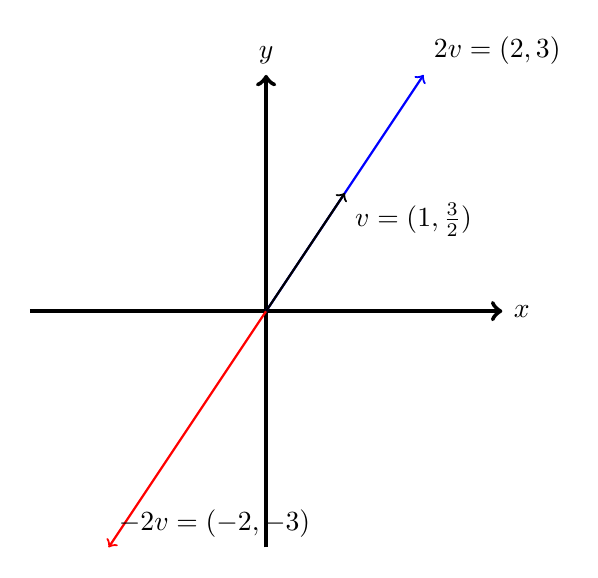
\begin{tikzpicture}
    \draw[->,ultra thick] (-3,0)--(3,0) node[right]{$x$};
    \draw[->,ultra thick] (0,-3)--(0,3) node[above]{$y$};

    % Vetor 2v
    \draw[->,thick, draw=blue] (0,0) -- (2,3) node[above right]{$2v=(2,3)$};
    % Vetor -2v
    \draw[->,thick, draw=red] (0,0) -- (-2,-3) node[above right]{$-2v=(-2,-3)$};
    % Vetor v=(1,2)
    \draw[->,thick] (0,0) -- (1,1.5) node[below right]{$v=(1,\frac{3}{2})$};
    \end{tikzpicture}
    \caption{Produto por escalar em $\mathbb R^2$.}
    \label{fig:produto-por-escalar}
\end{figure}
